\documentclass[UTF8,a4paper,zihao=5]{ctexart}

\usepackage[left=2.7cm,right=2.7cm,top=2.4cm,bottom=2.4cm]{geometry}
\usepackage{array,booktabs,tabularx,longtable}
\usepackage{graphicx}
\usepackage{listings}
\usepackage{xcolor}
\usepackage{amsmath}
\usepackage{enumitem}
\usepackage{hyperref}
\usepackage{caption}

\hypersetup{hidelinks}
\setlength{\parindent}{2em}
\setlength{\parskip}{0.25em}
\setlength{\emergencystretch}{2em}
\setlength{\tabcolsep}{5pt}
\renewcommand{\arraystretch}{1.25}
\pagestyle{plain}
\setlist{nosep,leftmargin=2em}
\lstset{
  language=Verilog,
  basicstyle=\ttfamily\footnotesize,
  columns=fullflexible,
  keepspaces=true,
  breaklines=true,
  showstringspaces=false,
  frame=single,
  rulecolor=\color{black!25},
  aboveskip=0.4em,
  belowskip=0.4em
}

\newcolumntype{C}{>{\centering\arraybackslash}X}
\newcommand{\reportsection}[1]{%
  \par\addvspace{0.75\baselineskip}%
  \noindent{\heiti\zihao{-4}#1\par}%
  \vspace{0.15\baselineskip}%
}
\newcommand{\code}[1]{\texttt{#1}}

\begin{document}

\begin{center}
  {\bfseries\zihao{3} 计算机组成原理实验课程第 6—7 次实验报告\par}
\end{center}
\vspace{0.3em}

\begin{center}
\begin{tabularx}{\textwidth}{|*{6}{C|}}
\hline
实验名称 & \multicolumn{3}{c|}{五级流水线 CPU 指令扩展与验证} & 班级 & 0965 \\
\hline
学生姓名 & 甘文杰 & 学号 & 2412700 & 指导老师 & 董前琨 \\
\hline
实验地点 & \multicolumn{2}{c|}{实验楼 A 304} & 实验时间 & \multicolumn{2}{c|}{2026 年 10 月 22 日} \\
\hline
\end{tabularx}
\end{center}

\reportsection{实验目的}
本实验在已有五级流水线 CPU 和 Lab3/Lab4 数据前递框架上，完成 Lab6 与 Lab7 的累计功能扩展。Lab6 主要加入算术逻辑指令、乘除法及 HI/LO 特殊寄存器操作；Lab7 继续加入控制转移、延迟槽和字节/半字/非对齐访存指令。实现时需要维持流水级握手、同步 RAM 时序和精确的写回边界，避免多周期运算期间重复接受或提交指令。

本次验收目标包括：按课程测试程序逐点检查 Lab6、Lab7；使用独立 CPU132 参考模型生成退休 trace 并与 DUT 比对；通过 HI/LO 单元级测试和除法期间分支等待定向用例补充检查；记录仿真周期、停顿、旁路使用和零号寄存器写回情况。

\reportsection{实验环境与总体设计}
实验使用 Vivado 2025.2、XSim 和 Windows 普通 PowerShell。Lab3 至 Lab7 共用一个 Vivado 工程，顶层为 \code{soc\_lite\_top}，仿真顶层为 \code{tb\_top}，目标器件为 \code{xc7a200tfbg676-2}。CPU 数据通路由 IF、ID、EX、MEM、WB 五级构成；IF 使用同步 ROM，MEM 连接 32 位数据 RAM。验证脚本在 Vivado 启动前检查执行环境，并为每轮仿真保留编译、展开、仿真阶段日志和结构化 \code{result.txt}。

图 1 是根据 RTL 接口和流水级职责绘制的结构示意图。图中前递回路、多周期 HI/LO 等待以及 MEM 字节通道用于解释设计关系；它是 Python 生成的说明图，不是 Vivado 仿真截图。完整流水级信号与模块边界仍以工程 RTL 为准。

\begin{figure}[htbp]
  \centering
  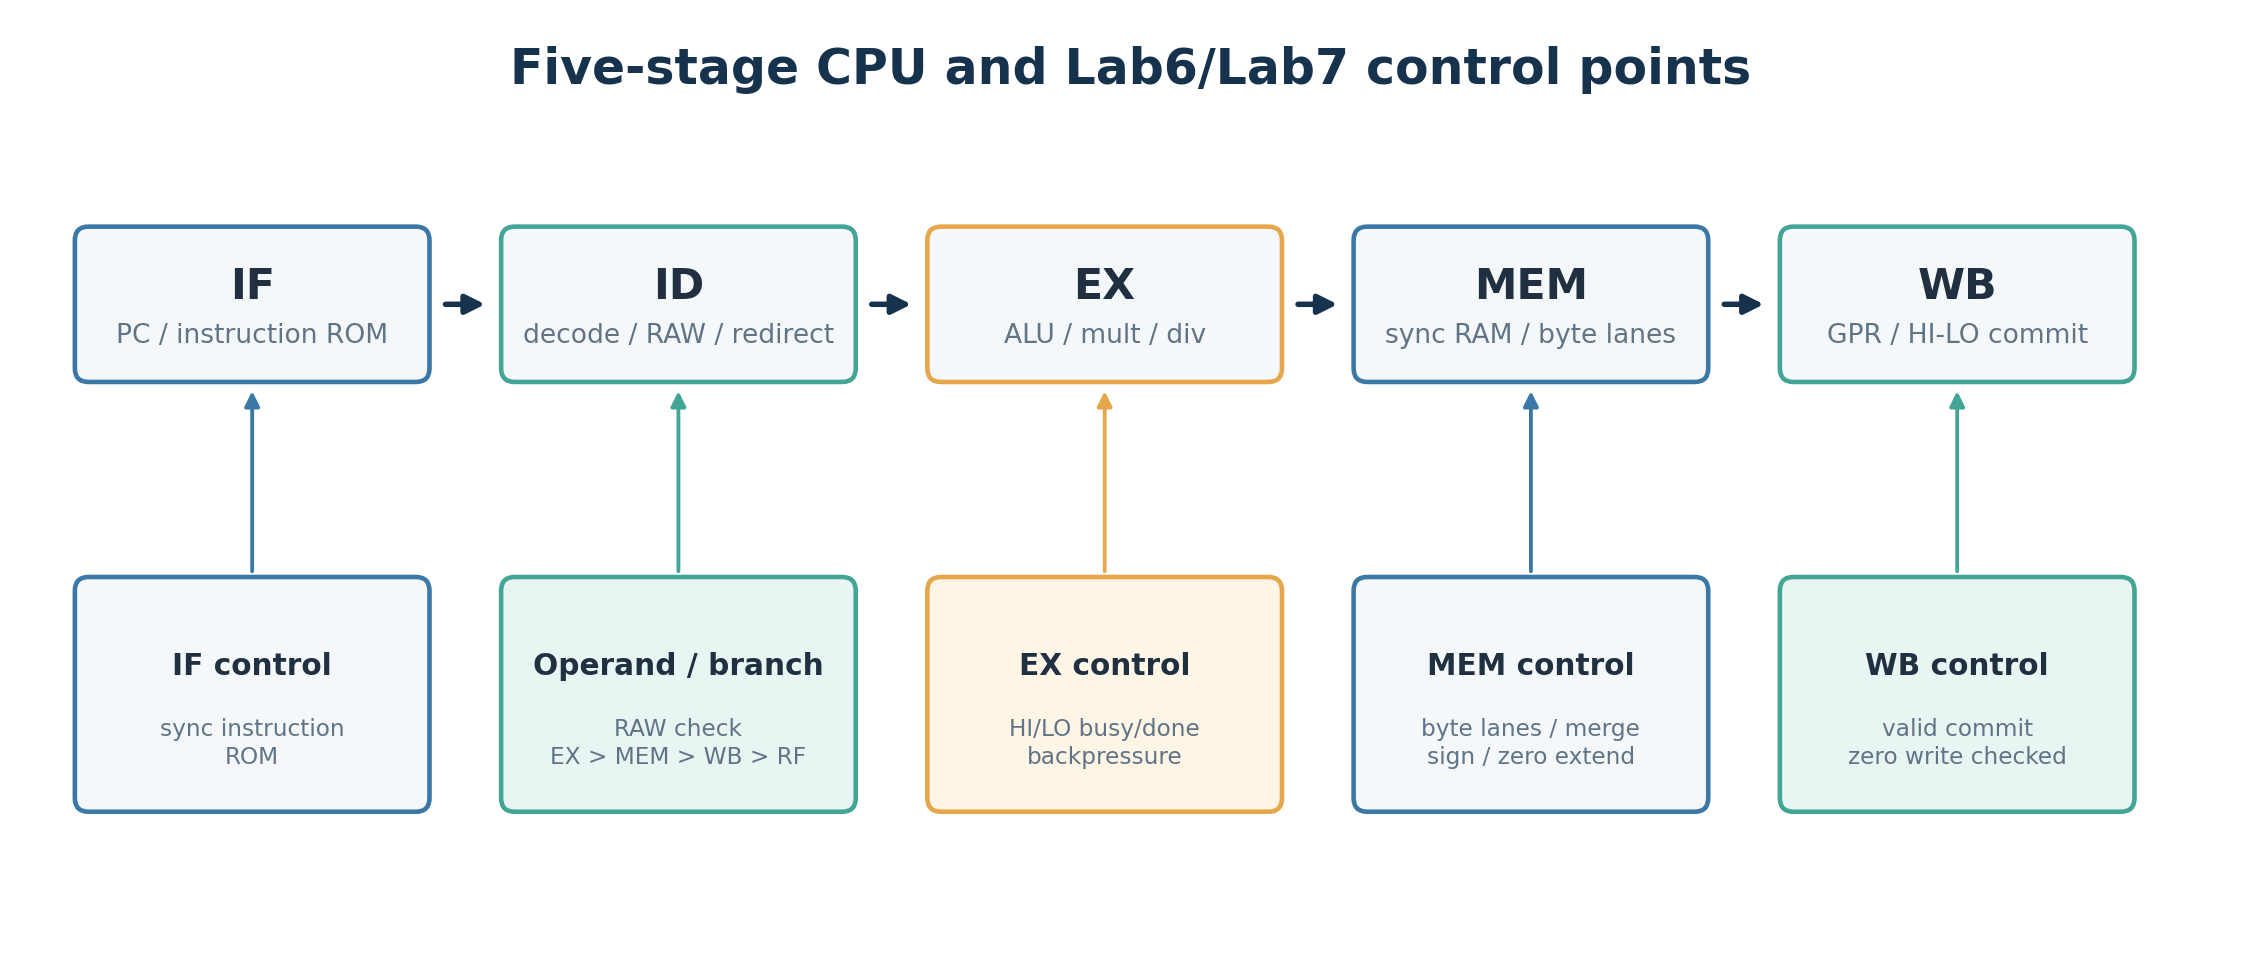
\includegraphics[width=0.98\textwidth]{figures/cpu_pipeline.png}
  \caption{五级流水线及 Lab6/Lab7 主要控制点（Python 绘制的结构示意图）}
\end{figure}

\reportsection{Lab6：算术逻辑与 HI/LO 扩展}
\textbf{算术逻辑指令。} ID 阶段增加 \code{add/sub/addi/slti/sltiu/andi/ori/xori/sllv/srav/srlv} 的译码，并相应确定源寄存器使用、目的寄存器和合法写回条件。EX 阶段对 \code{andi/ori/xori} 使用零扩展立即数，其余立即数按指令语义符号扩展；有符号比较与无符号比较分开处理。可变移位由 \code{rs[4:0]} 提供移位量、\code{rt} 提供被移位数据。

为避免未知或不支持编码造成伪写回，写回资格来自显式的合法指令集合，而不是仅凭某个译码位推断。新增 65-word 算术逻辑定向映像覆盖立即数边界、有符号/无符号比较、三种可变移位、高位移位量忽略、流水前递和 load-use。该定向 DUT 测试通过，73 周期、1 次 load-use 停顿，EX/MEM/WB 前递次数为 7/6/3，且 trace 与独立参考一致。

\textbf{HI/LO 运算。} 新增 \code{hilo\_unit.v} 封装乘法和除法 IP。乘法支持 signed/unsigned；除法器为 unsigned IP，signed 运算通过输入幅值化和输出符号恢复实现。乘法结果写为 HI=乘积高 32 位、LO=乘积低 32 位；除法结果写为 HI=余数、LO=商。\code{mfhi/mflo} 在 EX 使用 HI/LO 当前值，\code{mthi/mtlo} 在指令能够离开 EX 的提交边界更新特殊寄存器。

多周期乘除法在 EX 保持当前指令，\code{busy} 期间阻止更年轻指令越过；完成结果保持到 \code{consume\_done}，随后回到空闲态。\code{start} 仅在该指令有效、属于乘除法、且单元既不忙也未完成时发出。以下为实际 RTL 中关键握手的节选：

\begin{lstlisting}
assign es_hilo_start = es_valid && es_hilo_multdiv &&
                       !es_hilo_busy && !es_hilo_done;
assign es_hilo_consume = es_valid && es_hilo_done && ms_allowin;
assign es_ready_go = !es_hilo_multdiv || es_hilo_done;
assign es_allowin = !es_valid || es_ready_go && ms_allowin;
assign es_to_ms_valid = es_valid && es_ready_go;
\end{lstlisting}

图 2 展示单元请求、等待、完成保持和消费的状态关系。该图是依照 RTL 独立 testbench 观察到的握手绘制，图中状态名与实现一致。

\begin{figure}[htbp]
  \centering
  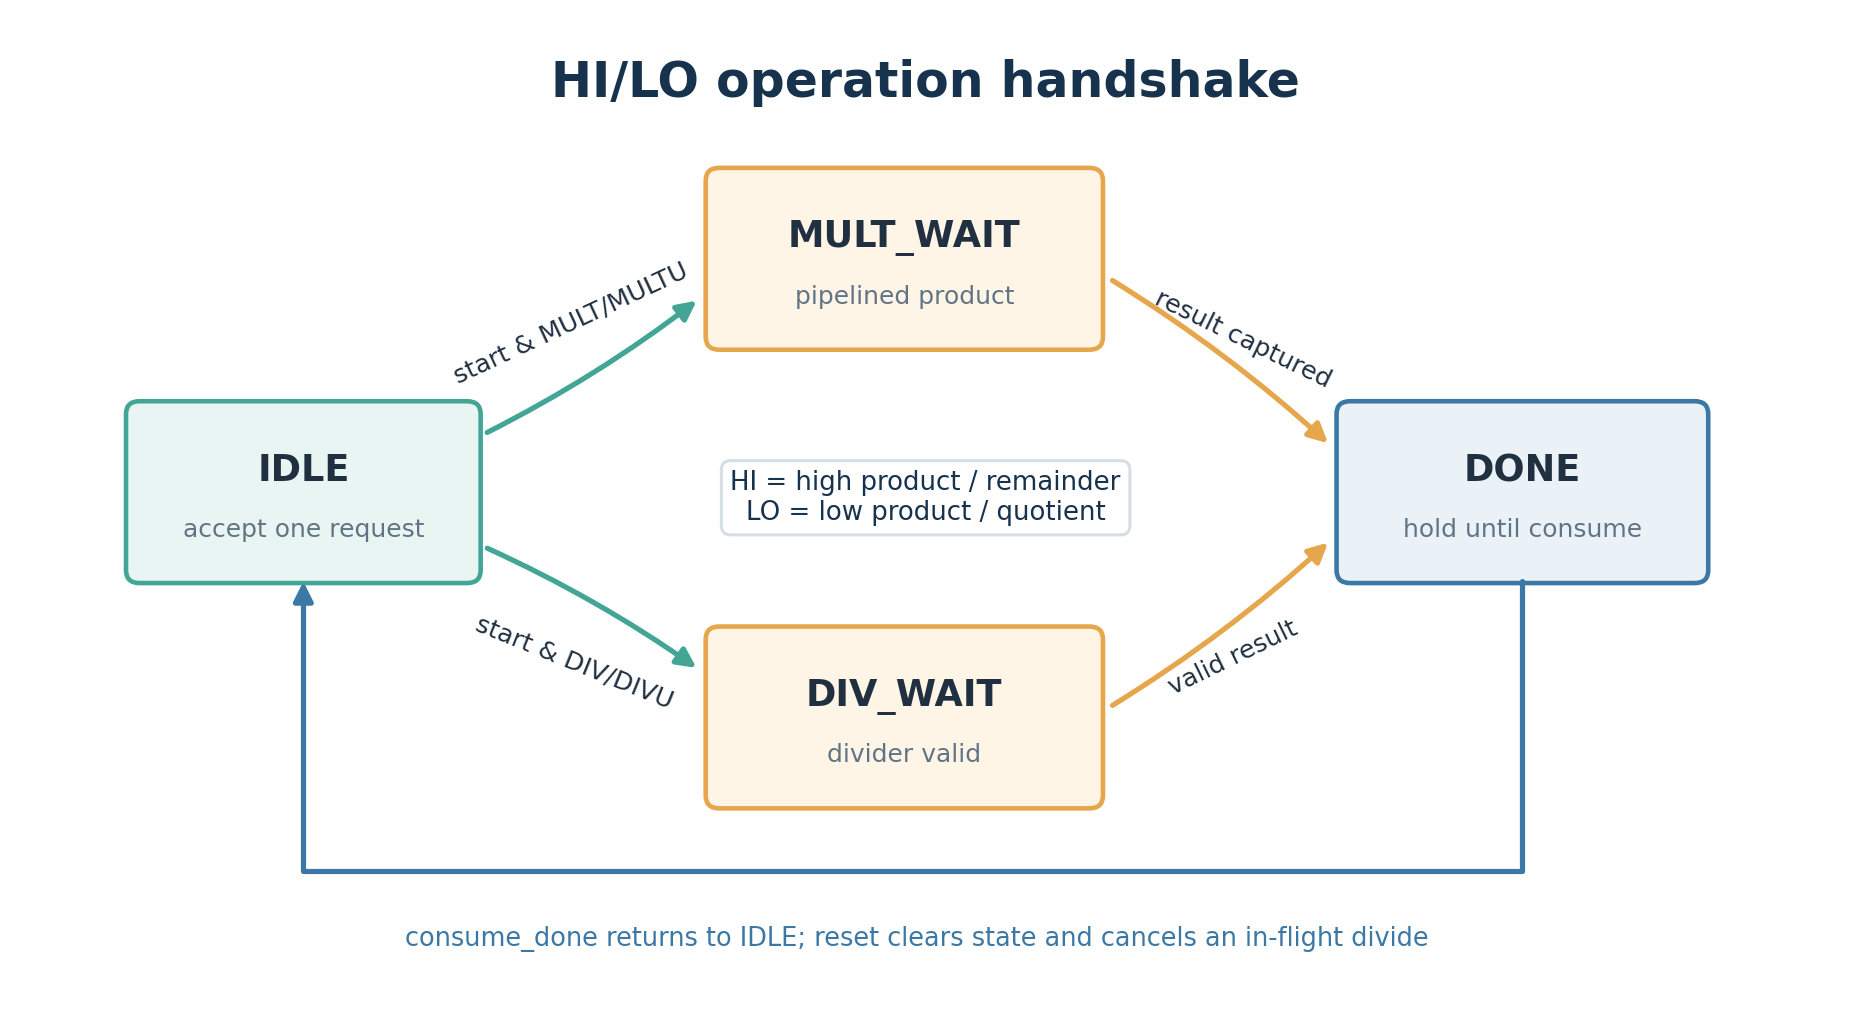
\includegraphics[width=0.83\textwidth]{figures/hilo_handshake.png}
  \caption{HI/LO 单元的请求与完成握手}
\end{figure}

\textbf{HI/LO 单元测试。} 独立 testbench 共接受 3 次乘法和 4 次除法请求，完成并提交 6 次；另有一次在完成前由复位取消。检查覆盖 signed/unsigned 运算、零乘数、完成保持直到消费、单次接受与单次提交、\code{MTHI/MTLO} 以及复位清除进行中的除法。testbench 通过。除法除数为零不属于本次已记录的测试覆盖，报告不据此推断其行为。

\reportsection{Lab7：控制转移、延迟槽与访存}
\textbf{控制转移。} 新增 \code{j}、\code{jalr}、\code{bgez/bgtz/blez/bltz} 和 \code{bgezal/bltzal}。条件分支按有符号 \code{rs} 判断；\code{jalr} 的目标来自经过前递的 \code{rs}，链接目的寄存器使用指令 \code{rd}。条件分支目标按 \code{PC+4+signext(imm<<2)} 计算，跳转目标使用 \code{(PC+4)[31:28]} 与索引字段拼接，链接值为 \code{PC+8}。\code{bgezal/bltzal} 的链接行为按课程测试宏要求，即使条件不成立也写链接值，是否重定向仍由条件决定。

分支仅在 ID 指令能够被 EX 接收时发出，保留一条延迟槽指令；若 EX 被多周期运算占用，ID 中的分支保持等待，不重复重定向。该路径使用独立定向程序验证：\code{DIV} 后紧接 taken \code{BEQ}，延迟槽写入 \code{r3=0x55}，fall-through 对 \code{r4} 的写入必须被跳过，分支目标后 \code{MFLO/MFHI} 分别读出商 $-4$ 和余数 $-3$，目标标记写入 \code{r7=0x66}。trace 中恰好出现 \code{r3/r5/r6/r7} 写回记录而没有 \code{r4} 写回记录，DUT 与独立参考 trace 全匹配。图 3 为该程序控制流的说明图。

\begin{figure}[htbp]
  \centering
  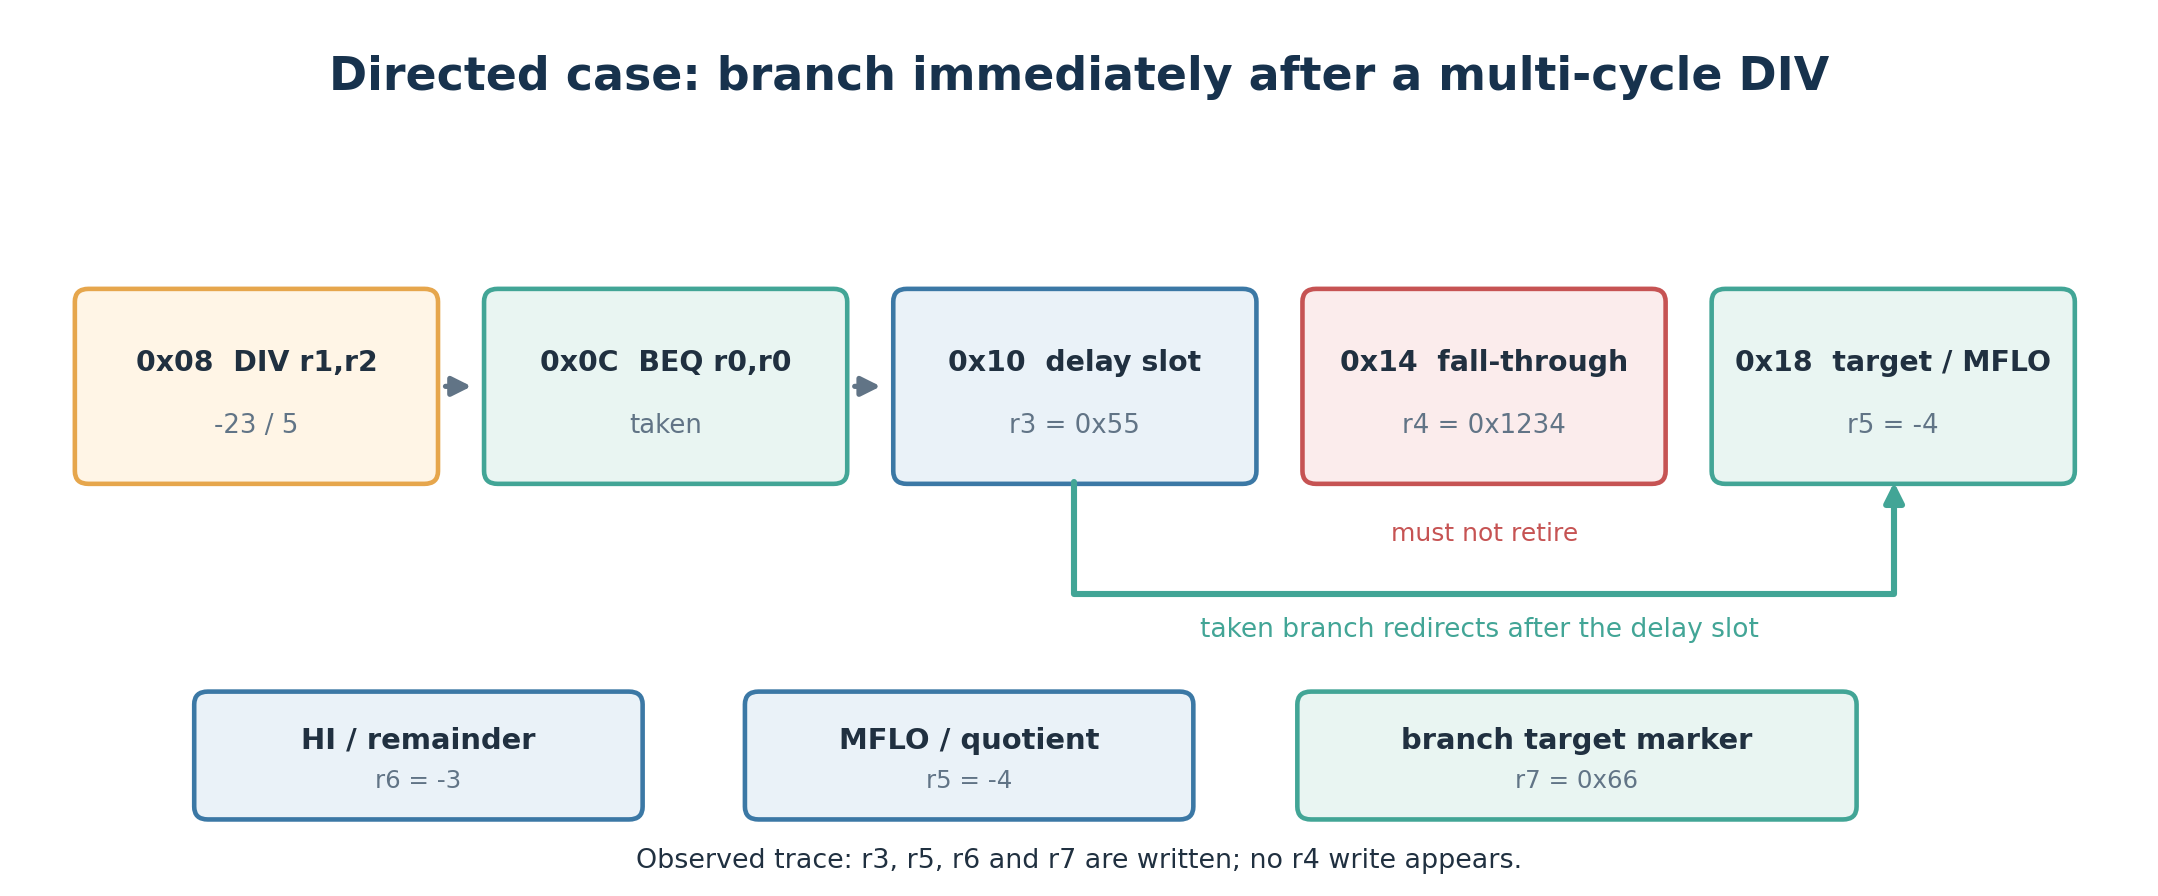
\includegraphics[width=0.98\textwidth]{figures/div_branch_delay_slot.png}
  \caption{除法占用 EX 时的分支等待、延迟槽和跳过路径定向检查}
\end{figure}

\textbf{访存指令。} 访存控制由单一 load/store 信号扩为 12 位 one-hot \code{mem\_op}，在一个字 RAM 接口上支持下表指令。地址按字索引访问 RAM，低地址位用于字节/半字通道选择；读数据由 MEM 阶段完成扩展或合并，写数据和 byte enable 在 EX 阶段按地址偏移生成。

\begin{center}
\small
\begin{tabularx}{\textwidth}{@{}>{\raggedright\arraybackslash}p{2.3cm}X X@{}}
\toprule
类别 & 指令 & 实现要点 \\
\midrule
整字 & \code{lw/sw} & 读写 32 位字，\code{sw} 的四个 byte enable 全开。 \\
字节 & \code{lb/lbu/sb} & 按地址低两位选 lane；\code{lb} 符号扩展，\code{lbu} 零扩展，\code{sb} 只使能目标 lane 并移位写数据。 \\
半字 & \code{lh/lhu/sh} & 用地址位 1 选择半字；load 分别进行符号扩展或零扩展，store 使能对应两个 lane。 \\
非对齐读 & \code{lwl/lwr} & 按低两位与旧 \code{rt} 合并；旧值来自经过 RAW 检测和前递的源操作数。 \\
非对齐写 & \code{swl/swr} & 按低两位生成写掩码和移位后的写数据。 \\
\bottomrule
\end{tabularx}
\end{center}

本实现沿用 32 位同步 data RAM，EX→MEM 总线增加有效地址和原 \code{rt} 值等信息。\code{lwl/lwr} 合并关系、\code{swl/swr} 四种偏移的掩码与数据排列已与独立 CPU132 reference 的执行级规则逐项核对。累计 Lab7 功能点回归通过并与 golden trace 匹配。

\reportsection{流水线接口与冒险处理}
Lab6/Lab7 在原 forwarding 流水线接口上继续传递新增控制和数据。\code{DS\_TO\_ES\_BUS\_WD} 扩为 154 位，\code{ES\_TO\_MS\_BUS\_WD} 扩为 114 位。普通数据相关使用 EX/MEM/WB 前递；HI/LO 运算通过 EX 的 ready/allow 握手施加多周期背压；同步 load 数据只有在 RAM 返回后才可用。零号寄存器始终不接受写回。

普通 RAW 前递按最近写者优先选择 EX、MEM、WB、寄存器堆。若最近写者匹配但结果尚未有效，消费者等待，不越过它去取更旧结果。这个优先级对 ALU 输入、分支比较、\code{jr/jalr} 目标以及 store 写数据保持一致。同步 RAM 的时序没有改变，因此 load-use 仍可能停顿；这是等待数据到达的必要等待，不作为普通 ALU 前递失败。

\reportsection{实验方法与验收规则}
累计课程映像的参考轨迹由独立 CPU132 参考环境生成；DUT 使用同一份 ROM MIF 运行 forwarding 模式。验收不仅检查 testbench 的功能点通过数，也检查参考 trace 是否打开、测试结束标记、PASS 标记、仿真退出码、使用的映像与源文件是否匹配，以及零号寄存器写回检查。每轮 Xvlog、Xelab、XSim 阶段的新鲜日志一并记录。

仿真周期数和停顿数直接引用该轮 \code{result.txt}。Lab6 与 Lab7 使用不同累计课程程序，因此二者周期数不能用来直接比较处理器性能。HI/LO testbench 和除法后分支程序作为补充覆盖；定向分支测试的课程功能点数为 0 是预期配置，它按自定义 trace 比较判定，不代表没有执行指令。

本报告未启用 Vivado 波形捕获。图 1—3 是结构/程序流程说明图，图 4 是由验收结果绘制的功能点汇总图，均不是仿真波形。运行脚本、trace、日志及哈希用于复核可重复性。

\reportsection{实验结果}
图 4 汇总 Lab6、Lab7 的累计课程功能点结果。详细数字和辅助检查见表 2。

\begin{figure}[htbp]
  \centering
  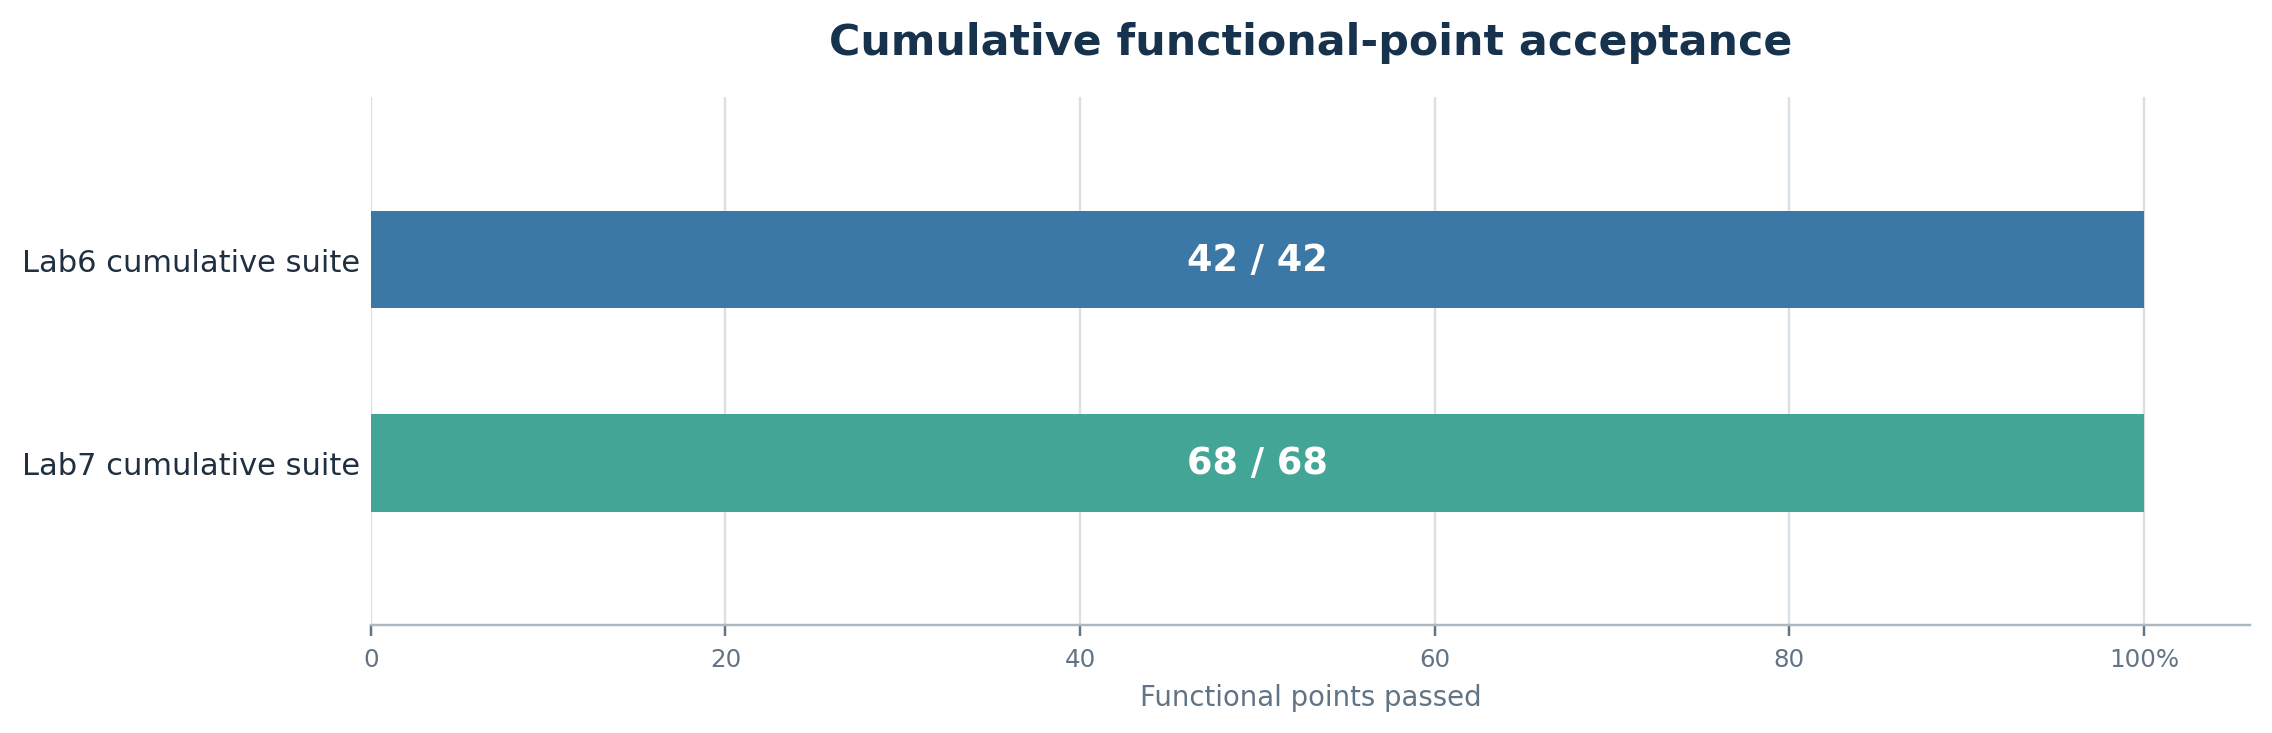
\includegraphics[width=0.82\textwidth]{figures/functional_coverage.png}
  \caption{Lab6 与 Lab7 累计课程功能点通过率}
\end{figure}

\begin{center}
\small
\begin{tabularx}{\textwidth}{@{}>{\raggedright\arraybackslash}p{3.35cm}*{2}{>{\centering\arraybackslash}X}@{}}
\toprule
指标 & Lab6 累计 & Lab7 累计 \\
\midrule
验收状态 & PASS & PASS \\
课程功能点 & 42/42 & 68/68 \\
流水线周期 & 109,375 & 166,226 \\
流水线停顿周期 & 89 & 926 \\
EX/MEM/WB 前递使用 & 35,013 / 8,320 / 12,007 & 49,970 / 12,229 / 15,454 \\
零号寄存器写回尝试 & 0（检查通过） & 0（检查通过） \\
trace 与 ROM 映像 & 哈希匹配 & 哈希匹配 \\
波形捕获 & 未启用 & 未启用 \\
\bottomrule
\end{tabularx}
\end{center}

Lab6 累计 trace 共 66,612 条记录，SHA-256 为 \code{FB92799C...6986850CA1}；使用的 MIF SHA-256 为 \code{E446C87C...D438AF46}。Lab7 累计 trace 共 100,732 条记录，SHA-256 为 \code{23ADD75B...B22035991C3}；MIF SHA-256 为 \code{4BCBB028...C223068C}。完整哈希、原始绝对路径和运行起止时间保存在对应 \code{result.txt}。

两轮累计 DUT 均在预期功能点数上全部通过，参考 trace 与仿真镜像匹配；zero-register 检查均报告 0 次实际写回尝试。HI/LO 单元 testbench 和除法期间分支等待定向用例也通过。旧的 S2 阶段 Lab6 结果曾在当时尚未实现 HI/LO 的 \code{mflo} 处通过 34/42；它是中间阶段记录，不能代替当前完整 RTL 的 42/42 结果。

\reportsection{结果分析与局限}
Lab6 与 Lab7 的累计功能点均达到本轮设定的完整通过条件。不同数据路径都获得独立证据：算术逻辑定向程序检查立即数、比较和可变移位；HI/LO testbench 检查多周期单元握手；自定义分支测试检查除法背压期间的延迟槽和重定向；累计课程 ROM 检查完整功能点并与独立参考退休 trace 逐项匹配。

当前验收证明的是指定课程映像和已记录定向场景下的仿真行为，不等同于形式化证明，也不包含板上实测、综合后时序收敛或所有非法输入组合。特别是除数为零没有列入 HI/LO testbench 覆盖；本报告不对该情况作正确性结论。由于本轮未捕获波形，报告不提供 Vivado GUI 截图；用户若以后需要波形，可用已记录工程和脚本重新运行并启用 \code{-CaptureWaveform}。

\reportsection{总结}
本次完成了 Lab6 算术逻辑与 HI/LO 乘除法扩展、Lab7 控制转移与延迟槽扩展，以及 12 类整字、字节、半字和非对齐访存操作。多周期单元通过 EX 级背压和完成消费握手避免重复执行；控制转移在 EX 停顿时等待，并保留一条延迟槽；访存操作按地址低位处理 lane、符号扩展和合并。

最终 Lab6 forwarding 累计仿真通过 42/42 功能点，Lab7 通过 68/68；两轮 trace 与映像哈希匹配，HI/LO 单元测试与除法后分支定向 trace 也通过。以上结果支持本报告所述实现与验收范围内的功能正确性结论。

\clearpage
\reportsection{附录 A：复现命令与证据索引}
从仓库根目录 \code{C:\textbackslash Users\textbackslash lenovo\textbackslash Desktop\textbackslash Projects\textbackslash FPGA\textbackslash lab} 的普通 Windows PowerShell 运行：

\begin{lstlisting}[language=bash]
powershell.exe -NoLogo -NoProfile -ExecutionPolicy Bypass `
  -File .\scripts\verify.ps1 -Case lab6 -PipelineMode forwarding
powershell.exe -NoLogo -NoProfile -ExecutionPolicy Bypass `
  -File .\scripts\verify.ps1 -Case lab7 -PipelineMode forwarding
\end{lstlisting}

Vivado 不应从 AppContainer 受限 PowerShell 启动。仓库脚本会在 Vivado 启动前检查当前 token，并记录 host context。报告配套图可在仓库根目录用下列命令重新生成（需安装 Python 与 Matplotlib）：

\begin{lstlisting}[language=bash]
python .\report\lab6-7\scripts\build_figures.py
\end{lstlisting}

\small
\begin{longtable}{@{}>{\raggedright\arraybackslash}p{3.5cm}>{\raggedright\arraybackslash}p{11.1cm}@{}}
\caption{报告结论对应的原始证据}\\
\toprule
报告内容 & 仓库内证据 \\
\midrule
\endfirsthead
\toprule
报告内容 & 仓库内证据（续） \\
\midrule
\endhead
Lab6 累计 DUT & \url{results/lab6_lab7/lab6-20261022T062908Z/result.txt}；同目录 Xvlog/Xelab/XSim 阶段日志。 \\
Lab7 累计 DUT & \url{results/lab6_lab7/lab7-20261022T063433Z/result.txt}；同目录 Xvlog/Xelab/XSim 阶段日志。 \\
HI/LO 单元 testbench & \url{results/lab6_lab7/hilo-unit-20261022T062119Z/result.txt} 与同目录日志。 \\
除法期间分支定向用例 & \url{results/lab6_lab7/directed/hilo-stall-branch/} 下程序映像及 golden trace；DUT 结果为 \url{results/lab3_lab4/lab3-20261022T065139Z/result.txt}。 \\
算术逻辑定向用例 & \url{results/lab6_lab7/directed/alu/} 和 \url{results/lab3_lab4/lab3-20261021T140840Z/}。 \\
实现记录 & \url{docs/lab6_lab7/implementation.md}。 \\
完整验收与哈希 & \url{docs/lab6_lab7/verification.md}。 \\
环境和运行入口 & \url{docs/lab6_lab7/environment.md}。 \\
\bottomrule
\end{longtable}

\normalsize
\end{document}
